\documentclass[border=2pt]{standalone}
\usepackage{tikz}
\usetikzlibrary{automata,arrows.meta}

\begin{document}
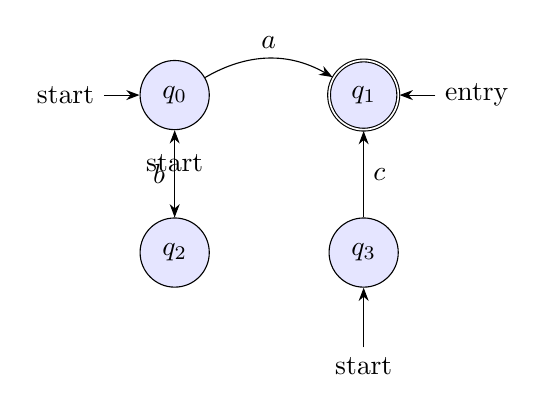
\begin{tikzpicture}[>=Stealth,every state/.style={fill=blue!10}]
  \node[state,initial] (q0) at (0,0) {$q_0$};
  \node[state,accepting,initial right,initial text=entry] (q1) at (2.4,0) {$q_1$};
  \node[state,initial above] (q2) at (0,-2) {$q_2$};
  \node[state,initial below,initial distance=5ex] (q3) at (2.4,-2) {$q_3$};
  \path[->] (q0) edge[bend left] node[above] {$a$} (q1)
             (q2) edge node[left] {$b$} (q0)
             (q3) edge node[right] {$c$} (q1);
\end{tikzpicture}
\end{document}
